% Created 2018-02-19 Mon 05:04
\documentclass{article}
\usepackage[mathletters]{ucs}
\usepackage[utf8x]{inputenc}
\usepackage[T1]{fontenc}
\usepackage{fixltx2e}
\usepackage{graphicx}
\usepackage{longtable}
\usepackage{float}
\usepackage{wrapfig}
\usepackage{rotating}
\usepackage[normalem]{ulem}
\usepackage{amsmath}
\usepackage{textcomp}
\usepackage{marvosym}
\usepackage{wasysym}
\usepackage{amssymb}
\usepackage{hyperref}
\tolerance=1000
\date{\today}
\title{Notebook3}
\hypersetup{
  pdfkeywords={},
  pdfsubject={},
  pdfcreator={Emacs 25.3.1 (Org mode 8.2.10)}}
\begin{document}

\maketitle
\tableofcontents

\section{Information and Pitfalls in Feature detection}
\label{sec-1}

\begin{enumerate}
\item Misconceptions
\label{sec-1-1}
\begin{itemize}
\item I wrongly misconstrued what Ι had to do with this assignment, I had
two wrong starts.
\begin{enumerate}
\item I thought Ι had to use Fast/Discrete Fourier Transformers.
\item I thought I had to implement the SIFT algorithm.
\end{enumerate}
\item Due to these Misconceptions I have some insights with these two approaches
\item I eventually ended up on the discrete correlation algorithm which
relied on convolutions.
\end{itemize}
\item Fourier Transformers what are they
\label{sec-1-2}
\begin{itemize}
\item A Fourier Transformer can be thought of as a formula that
transformers a wave into the components that make up said wave.
\item For a concrete example, let's say that we wish to find out the
ingredients of a drink
\begin{itemize}
\item The Fourier transformer would allow us to split the drink into the
base components (signals).
\item Note with this example, we can easily see that we can combine all
the ingredients of the drink and get back our original drink. This
is important because the Fourier Transformer has an inverse
function, meaning that we can get our original signal back
\end{itemize}
\item Fourier Transformations are used for this as it can reduce a
complex convolution like operation (cross correlation) into a few
transformations and a single matrix multiplication
\end{itemize}
\begin{enumerate}
\item Discrete Fourier Transformer
\label{sec-1-2-1}
\begin{itemize}
\item Fourier Transformers are defined on continuous space, however we
wish to do these operations on an image, so we need to do this over
a \textbf{discrete} domain
\begin{itemize}
\item The formula for the Discrete Fourier transformer is listed below,
note that this formula is run on complex numbers
\item X$_{\text{K}}$ = $\sum$$^{\text{N-1}}_{\text{n=0 }}$x$_{\text{n}}$×e$^{\text{-i2πkn/N}}$
    where \{x$_{\text{n}}$\} = x$_{\text{0}}$,\dots{},x$_{\text{N-1}}$
\item This transformation will be denoted with F
\item Notice that each computation of X$_{\text{k}}$ takes N computations, leaving
the entire operation at O(N$^{\text{2}}$)
\end{itemize}
\end{itemize}
\item Fast Fourier Transformer
\label{sec-1-2-2}
\begin{itemize}
\item This is just a way computing the Discrete Fourier
Transformer in O(N log(N)) instead of O(N$^{\text{2}}$)
\item However there are some caveats, The variation used in Haskell's Repa
library uses Cooley-Tukey algorithm which requires that N is a power
of two as it's a divide and conquer algorithm which splits the problem
into 2's.
\item This means that in order to use a Fast Fourier Transformer, one must
convert their image into a power of two
\end{itemize}
\end{enumerate}
\item SIFT
\label{sec-1-3}
\begin{itemize}
\item SIFT stand for Scale invariant feature transform, and there are many
similar algorithms which preform better (such as speeded up robust
features (SURF)).
\item SIFT is more robust than what I ended up going with as it resistant
to illumination changes and to a lesser degree affine changes, which
would allow it to match many of the images seen in slide 2 and 3 of
Lecture 4.
\begin{itemize}
\item Affine transformation is a mapping f : X → Y where X and Y are
Affine spaces s.t f(x) = Mx + b.
\item Basically these transformations preserve straight lines and plane.
\end{itemize}
\end{itemize}
\item Discrete Cross Correlation
\label{sec-1-4}
\begin{itemize}
\item I ended up on implementing the two dimensional cross correlation, as
I found it rather easy to comprehend (though a bit hard to compute
with my tools).
\item This Calculation can be thought of the convolution of a kernel over
an image divided by the square root of the matrix Multiplication of
the kernel squared times the square of the matrix multiplication of
the vector the kernel is over.
\begin{itemize}
\item This can be expressed as $r(x,y) = \frac{\sum_{x',y'}(Img(x',y') × Ker(x + x', y + y'))^2}{\sqrt{\sum_{x',y'}(Img(x',y')^2 × \sum{x',y'}(Ker(x + x', y + y')^2)))}}$
\item Intuitively this makes sense as a cross correlation, as if the
image and kernel are similar at a sub-matrix, then that value would
be close to one, and if they are further apart, the division would
go towards closer to 0
\end{itemize}
\end{itemize}
\end{enumerate}
\section{Implementation of feature Detection}
\label{sec-2}
\begin{enumerate}
\item Lessons Learned
\label{sec-2-1}
\begin{itemize}
\item Not using a Fourier Transformer for a Cross Correlation is horribly
slow, where even a 200x200\textasciitilde{} image with a 25x25\textasciitilde{} pixel takes around
30 seconds to compute and a 1200x800 image with a 112 x 107 kernel
takes 30 minutes to compute
\item Also the Cross Correlation on its own is rather frail, or I ended up
screwing up the logic on it
\end{itemize}
\item By hand
\label{sec-2-2}
\begin{itemize}
\item My very first attempt was rather silly, as Ι just took the
convolution of two images, I won't say much more, outside of my
first attempt being a failure.
\item My second attempt ended up implementing the Cross Correlation,
however Ι needed to setup some tools first before Ι can compute it
\begin{itemize}
\item My first tool was padArray, as I can't just rely on the
convolution tool Ι ended up relying on for all previous computations
\begin{verbatim}
padArray :: Source r e ⇒ Int → Int → Array r DIM2 e → Array D DIM2 e
padArray row col arr = R.backpermute (Z :. i + 2 * row  :. j + 2 * col)
                                     getClosest arr
  where
    Z :. i :. j = R.extent arr
    getClosest (Z :. row' :. col') = ix2 roff coff -- col' - col is for getting
     where coff = min (max (col' - col) 0) (i - 1) -- the pos in the old array
           roff = min (max (row' - row) 0) (j - 1) -- from the new coordinates
\end{verbatim}
\begin{itemize}
\item This function takes an array and creates a new array with the top
and sides padded by that amount.
\end{itemize}
\item With this tool in hand we can compute the normalizedConvolution
\begin{verbatim}
normalizedConv :: Array r DIM2 Double → Array U DIM2 Double → m (Array U DIM2 Double)
normalizedConv arr ker = do
  let Z :. ik :. jk = R.extent ker
  arrExtended      ← R.computeUnboxedP $ padArray (ik `div` 2) (jk `div` 2) arr
  normKern         ← mmultP ker ker
  let normKernSum   = normKern `deepSeqArray` sumAllS normKern
  let extracted     = repaExtractWindows2D ik jk arrExtended
  let fn subarr     = sumAllS (subComp *^ ker) 
                      / √ (normKernSum * sumAllS (mmultS subComp subComp))
        where subComp = computeUnboxedS subarr
  R.computeUnboxedP $ R.map fn extracted
\end{verbatim}
\begin{itemize}
\item This function is a bit more involved, however it should
resemble the verbal description of the cross correlation in
section 1.
\item The functions that end in P get processed in parallel, as being
parallel on such a slow algorithm is paramountl
\item extractWindows2D is how I get an array with subarray the same
size as our kernel, I run this on the padded array, as from here
we can just apply the cross correlation algorithm.
\end{itemize}
\item Now that we have our normalizedConvolution function, we can now
calculate the imageCorrelation.
\begin{verbatim}
imageCorrelation ::  Double → FilePath → FilePath → IO (Array U DIM2 Double)
imageCorrelation min path1 path2 = do
  x     ← readIntoRepa path1 >>= toGreyP
  y     ← readIntoRepa path2 >>= toGreyP
  let x' = R.map fromIntegral x
  y'    ← R.computeUnboxedP $ R.map fromIntegral y
  convd ← normalizedConv x' y'
  computeUnboxedP $ transpose $ filterMin convd min
\end{verbatim}
\begin{itemize}
\item Here we load the two images and turn them grey.
\item Then we just normalize the two functions and remove all pixels
that are below a certain value.
\end{itemize}
\item We can now run this algorithm. Sadly this algorithm doesn't
actually produce the results we want.
\begin{itemize}
\item I ran the kernel on the single soccer ball seen below on the
image full of soccer balls
\item The output is the black and white blob which is obviously an
incorrect detection. Furthermore it is all black if Ι turn the
measly 0.012 minimum value to 0.02
\begin{figure}
  \centering
  \begin{subfigure}
    \centering
    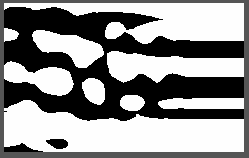
\includegraphics[width=.4\textwidth]{../data/object/ImageTest.png}
  \end{subfigure}
  \begin{subfigure}
    \centering
    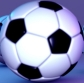
\includegraphics[width=0.4\textwidth]{../data/object/soccer-kernel1.jpg}
  \end{subfigure}%
  \begin{subfigure}
    \centering
    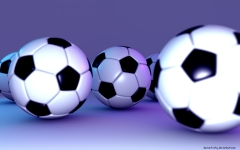
\includegraphics[width=0.4\textwidth]{../data/object/soccer_balls1.jpg}
  \end{subfigure}%
\end{figure}
\end{itemize}
\end{itemize}
\item Sadly Ι haven't figured out what went wrong in my algorithm. It
might just be the case that the cross correlation algorithm is not
supposed to used in such a matter and is thus rather frail for what
I'm trying it for.
\end{itemize}
\item OpenCV
\label{sec-2-3}
\begin{itemize}
\item This implementation had it's own set of pains, which will bet
discussed more at the end.
\item I'm still not fully sure how to manipulate the Mat data structure
provided by OpenCV.
\begin{verbatim}
cvMatrix8 = fmap (fromImage . extractLumaPlane) . loadRGBJPG

cvMatrix16 = fmap (fromImage . extractLumaPlane) . loadRGB16


correlate arr ker = do
  arr' <- cvMatrix8 arr
  ker' <- cvMatrix8 ker
  let correlation = runExcept $ matchTemplate arr'
                                              ker' 
                                              MatchTemplateCCoeff
                                              MatchTemplateNormed
  case correlation of
    Left _ -> error "erorr in transformation"
    Right m -> CV.withWindow "test" $ \win -> CV.imshow win arr'
\end{verbatim}
\begin{itemize}
\item thankfully Haskell's OpenCV offers me a frmImage function which
allows me to transform my image into a openCV format.
\item I've tried a byte String transformation as well, but sadly that
caused issues with the matchTemplate function openCV provides.
\item the correlate function is where the magic occurs, as we read in an
array and a kernel and computes the cross correlation between
them. Note that this is the same algorithm as the one I outlined
above, however there are many variations that openCV is willing to
work with
\item from here we just read the correlation into an openCV window where
it is supposed to be displayed.
\begin{itemize}
\item I couldn't easily turn this back into an image due to the double
type and my inability to try to coerce the type
\end{itemize}
\item Sadly, it seems the openCV bindings given are broken (at last on
my machine), as cvMatrix8 actually gives me an array out of bounds
errors for whatever reason, and Ι don't see an easy way to fix
it. So sadly this approach too leads in failure
\end{itemize}
\end{itemize}
\end{enumerate}
% Emacs 25.3.1 (Org mode 8.2.10)
\end{document}